\documentclass{article}
\usepackage{graphicx}
\usepackage{hyperref}
\usepackage{url}

\setlength{\parskip}{1em}

\begin{document}


\title{Visualizing Output}

Currently, ICE features two plugins for visualizing and plotting simulation
output data:

\textbf{VisIt Tools} - An interactive 3D visualization tool for rendering
meshes, scalar plots, contour plots, and more. 

\textbf{CSV Plotting Tools} - A customizable, 2D data plotting utility for data 
from .csv files.

\section{Installation and Configuration}

The CSV Plotting Tools require no additional software or preparation before use.
The VisIt Tools need both an instance of VisIt and a connection between ICE and
the VisIt session.

\subsection{VisIt Installation} 

Before preparing ICE,
\href{https://wci.llnl.gov/simulation/computer-codes/visit/}{VisIt}, developed
by Lawrence Livermore National Laboratory, must be downloaded. This must be
version 2.8.2 or higher, and does not need to be on the same machine that ICE is
installed on, as ICE is capable of launching a VisIt session on a remote machine. Make
note of the folder where you installed VisIt for use in the next step.

\subsection{Configuring the VisIt Connection}

Once VisIt is installed, ICE must connect to a VisIt session in order to provide
data visualization. There are two different parts of ICE which connect with
VisIt, both providing slightly different functionalities. These are the Plot
Editor, which is slightly more user friendly, and the Visualization Perspective,
which allows for arbitrary Python commands to be sent to the VisIt client. 

\subsubsection{Connecting for the Plot Editor} 

This process will set up a default connection to VisIt in the ICE Preferences
page, and so only needs to be performed once. After creating the connection, ICE
will launch and connect with VisIt each time it is started.

To set the connection, select Window $\rightarrow$ Preferences in ICE's
toolbar. (If you are using Mac OSx, this will instead be located at Eclipse
$\rightarrow$ Preferences.) Then select Visualization $\rightarrow$ VisIt in the
tree of the Preferences page.

\begin{center}
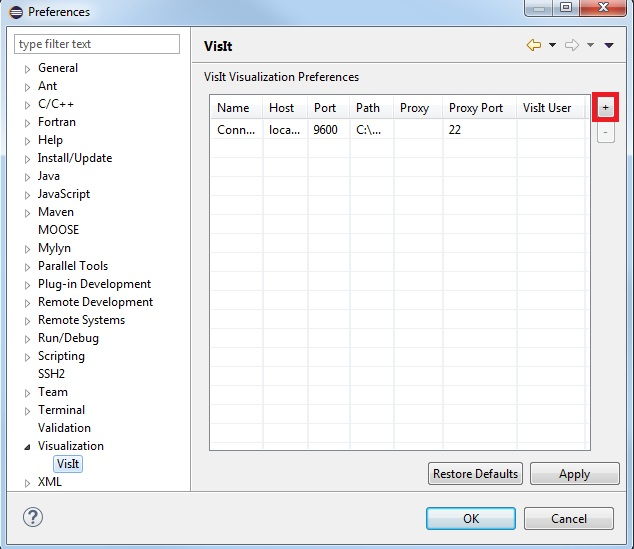
\includegraphics[width=12cm]{images/VisItPreferencePage_ICE}
\end{center}

Press the new row button, the button with a "+" symbol in the upper right,
highlighted in the image above. You can then click on each of the cells of the
new row to edit them. The default values automatically supplied by ICE should
be fine for most users. However, two fields may need to be changed:

\textbf{Host:} The default value of "localhost" is for connections to local
installations of VisIt on your computer. If you want to launch a remote VisIt
connection, you must change this to the hostname of the machine to connect to.

\textbf{Path:} You need to put the full path to the VisIt folder here. The path
should end with the folder containing the VisIt executable. For example, if
VisIt.exe is in a folder called VisIt 2.9.1, the the path should end in
\textbackslash{}VisIt 2.9.1\textbackslash , not \textbackslash{}VisIt
2.9.1\textbackslash VisIt.exe.

Once finished, press Apply, then OK. ICE will then open VisIt and connect to it.

\subsubsection{Connecting for the Visualization Perspective} 

First, open the Visualization perspective. On the main menu bar at the top of
the window, click Window $\rightarrow$ Perspective $\rightarrow$ Open
Perspective $\rightarrow$ Other\ldots, select Visualization in the dialog that pops up and click OK.
Alternatively, you can also access the same pop-up dialog by clicking the Open Perspective button in
the main toolbar in the upper right-hand corner of the ICE workbench. 

\begin{center}
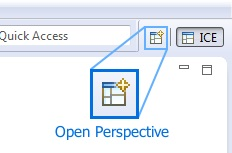
\includegraphics{images/ICE_OpenPerspective}
\end{center}

Now click the Launch VisIt button in the menu bar.

\begin{center}
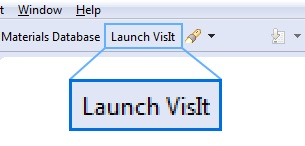
\includegraphics{images/ICE_VisItLaunchButton}
\end{center}

This will open a dialog offering you three options for connecting to VisIt.

\begin{center}
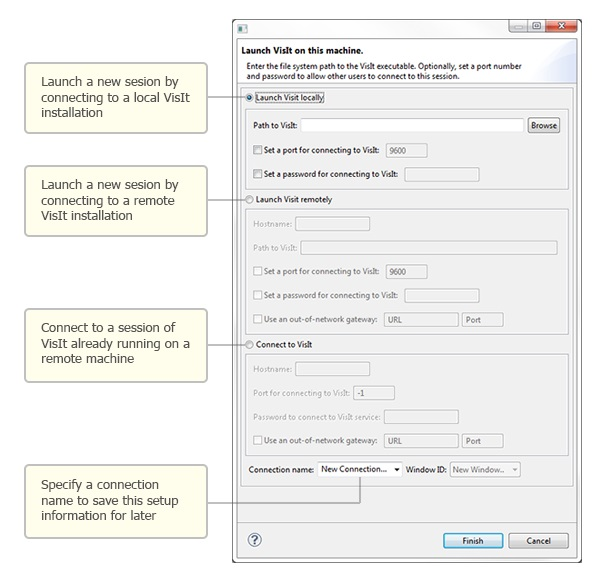
\includegraphics[width=12cm]{images/ICE_VisItLaunchOptions}
\end{center}

\textbf{1) Launch VisIt locally -} If you installed VisIt on your local machine,
use the Browse button to direct ICE to your local installation directory. Using this
method of connecting will launch a new VisIt session. Optionally, you can also
set a port number (default 9600) and--if you want to share your VisIt session
with another user--a password.

\textbf{2) Launch VisIt remotely -} If you installed VisIt on a remote machine,
specify the hostname and full path to the VisIt installation directory. Using this
method of connecting will launch a new VisIt session. Optionally, you can
specify a port number (default 9600) and--if you want to share your VisIt
session with another user--a password. If you need or want to use an external
gateway or proxy to access the remote VisIt installation, you may specify its
URL and port number as well.

\textbf{3) Connect to VisIt -} If you would like to connect to a session of VisIt
already running somewhere else, specify the hostname, port number, and password set on
the VisIt session; you will need to obtain this information from the person who
initially launched the VisIt session. If you need or want to use an external
gateway or proxy to access the remote VisIt installation, you may specify its
URL and port number as well.

If you've forgotten where VisIt is installed on Windows, find a shortcut to
VisIt either on your desktop or in the start menu. Right-click the shortcut and
open its Properties. The path to the VisIt executable's directoy will be shown
next to Target.

Regardless of which method you choose to connect to VisIt, enter a Connection
name at the bottom of the pop-up dialog. 

If you are connecting to an existing session, specify a Window ID between 1 and
16. Which Window ID you use depends on how you would like to connect to VisIt.
If multiple users connect using the same Window ID, they will all see and be
able to interact with the same VisIt view. However, if you would like multiple
users to each have their own unique session each with its own controls, assign a
unique Window ID to each user. The VisIt installation can support up to 16
unique window IDs at a time.

Once you are done, click the Finish button at the bottom, and ICE should begin
connecting to VisIt.

\section{VisIt}

\subsection{Opening a VisIt File}

\subsubsection{Opening a Plot Editor} 

To open a plot editor, first the file must be placed in the Project Explorer.
This view lists files imported into ICE. To access the Project Explorer, use the
the main menu bar at the top of the window and navigate to Window $\rightarrow$
Show View $\rightarrow$ Project Explorer. 

By default, the Project Explorer should automatically import the
ICEFiles/default and ICEFiles/itemDB folders. If it does not, or it you want to
import a different folder into ICE, right click in the Project Explorer and
select Import... from the context menu. Then select General $\rightarrow$ File
System from the tree and press the Next button. You can then select directories
and/or files to import into the Project Explorer and which folder they should be
imported under, as seen below.

\begin{center}
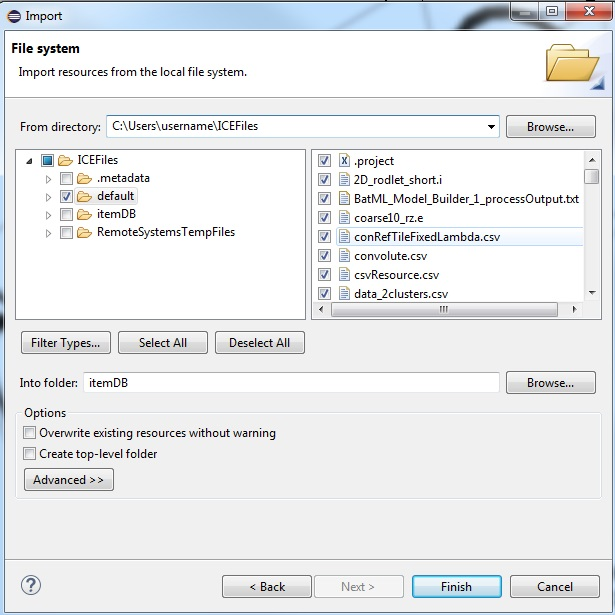
\includegraphics[width=12cm]{images/ImportFileDialog}
\end{center}

Once a file is in the Project Explorer, you can simply double click on it to 
open it in VisIt.

\subsubsection{Opening in the Visualization Perspective}

\begin{center}
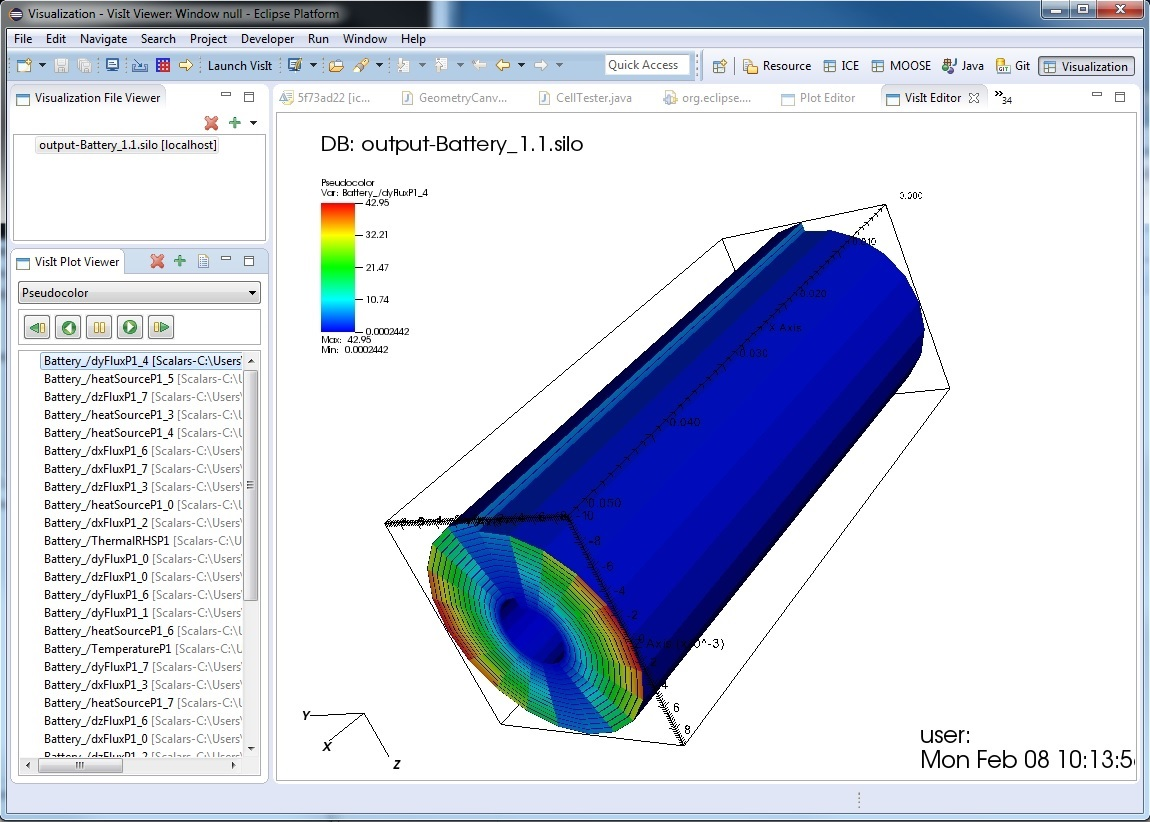
\includegraphics[width=12cm]{images/VisualizationPerspectiveOverview}
\end{center}

To open a file in the Visualization Perspective, it must first be imported into
the Visualization File Viewer, located in the upper left of the screen. To do
this, click the Open a File button, with a green plus sign icon. This will open
a dialog to let you select a local file to import.

\begin{center}
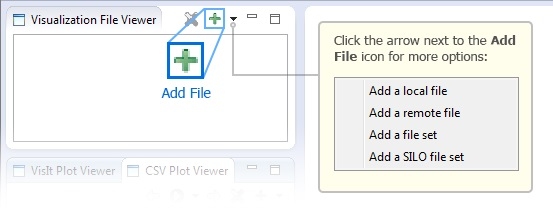
\includegraphics[width=12cm]{images/VisualizationAddFile}
\end{center}

Currently, ICE can only open files in VisIt on the same machine as that VisIt
session is running. If you are connected to a remote VisIt installation, you
will instead need to click the arrow beside the Open a File button and select
``Add a remote file'' from the drop down menu. This will open a dialog box to
browse the file system of the remote machine VisIt is hosted on, which can be
used to select a file as normal.

\begin{center}
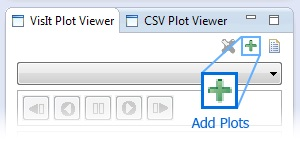
\includegraphics[width=12cm]{images/VisualizationAddPlots}
\end{center}

Once your file is in the Visualization File Viewer, you will need to create a
plot from it. To do this, select the file and then click the Add a Plot to the
List button located in the VisIt Plot Viewer on the left of the screen. A window
will open, prompting you to select which plots from the file you would like
to view. After you have made your selection and hit OK, these plots will be
placed in the VisIt Plot Viewer.

\begin{center}
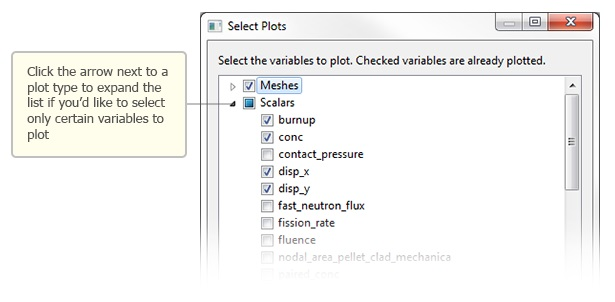
\includegraphics[width=12cm]{images/VisualizationSelectPlots}
\end{center}

Finally, you may double click a plot in the VisIt Plot Viewer to open that plot
in VisIt. 

\subsection{Using VisIt}

Both methods of accessing VisIt allow the user to rotate the model by clicking
and dragging inside the display area or zoom it by scrolling the mouse wheel.
Other commands require slightly different actions between the two. 

\subsubsection{Selecting the Plot}

In the Plot Editor, pressing the Select Series\ldots button will open a dialog
which lists the various plots in the opened file. Simply select one and click OK
to open it. 

\begin{center}
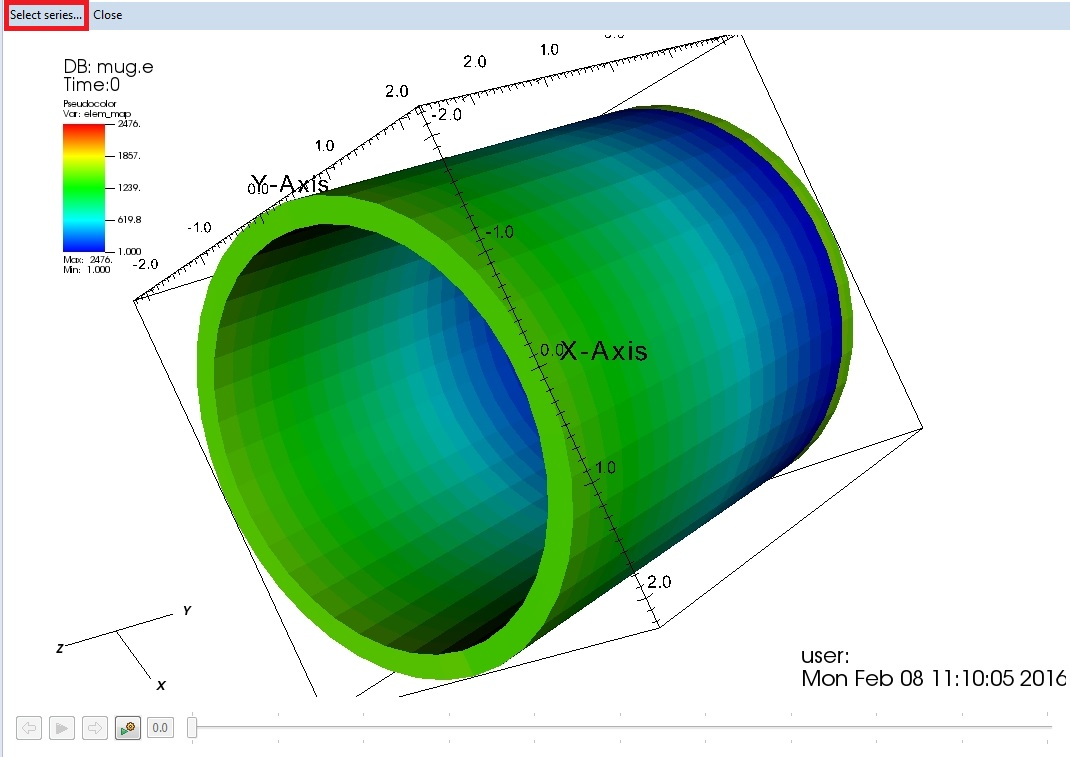
\includegraphics[width=12cm]{images/PlotEditorSelectSeriesButton}
\end{center}

In the Visualization Perspective, the opened plots will be listed in the VisIt
Plot Viewer. Double click on one to open it.

\subsubsection{Setting the Plot Representation}

VisIt is capable of displaying plots in several different representations, such
as pseudocolor, contour, or volume.

To switch between these in the Plot Editor, right click inside the display area
and select one of the listed options under the Representation category in the
context menu.

The Visualization Perspective features a drop down menu at the top of the VisIt
Plot Viewer which allows for switching between the available representations. 

\begin{center}
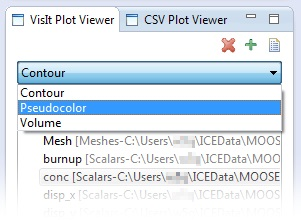
\includegraphics[width=12cm]{images/VisItRepresentationDropDown}
\end{center}

\subsubsection{Animation and Time Data}

The Plot Editor features a time slider widget at the bottom of the screen. 

\begin{center}

\includegraphics[width=12cm]{images/TimeSliderWidget}
\end{center}

The controls, in order of left to right, are:

1) Return to the previous time step.

2) Automatically play the plot as an animation by displaying the time steps
sequentially. 

3) Advance to the next time step. 

4) Opens an options menu that allows the user to set the playback speed, toggle
whether the animation should loop when it reaches the end, and set the plot to
the first or last time step.

5) A display for the current time step. It can be edited to set the plot to an
arbitrary time step. 

6) A slider that shows the current time step's position on the timeline. The
slider can be dragged around the timeline, setting the plot's time step
accordingly.

In the Visualization Perspective, the Visit Plot Viewer has a similiar set of
controls.

\begin{center}
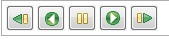
\includegraphics[width=12cm]{images/VizPerspectiveTimeControls}
\end{center}

The buttons, in order of left to right, are:

1) Return to the previous time step.

2) Automatically play the plot as an animation backwards, going through the time
steps in reverse order.

3) Pause the animation.

4) Automatically play the plot as an animation by displaying the time steps
sequentially.

5) Advance to the next time step. 

\subsubsection{Sending VisIt Python Commands}

This functionality is only available in the Visualization Perspective.

\begin{center}
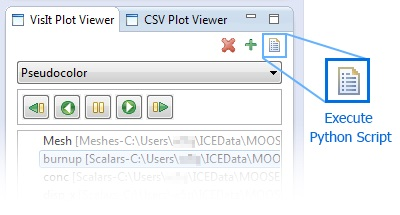
\includegraphics[width=12cm]{images/PythonScriptButton}
\end{center}

The Execute Python Script button in the upper right of the VisIt Plot Viewer
will open a new window with a Python shell. Commands entered into this shell
will be sent to the instance of VisIt. 

Python code can be written into the shell directly, but the Load from File
button will import an existing .py script into the console. Once done, hit the
Execute button to send the python command(s) to VisIt.

Writing Python scripts for VisIt is beyond the scope of this tutorial. However,
you are welcome to refer to the
\href{https://wci.llnl.gov/simulation/computer-codes/visit/manuals}{VisIt Python
Interface Manual} provided by the VisIt development team at Lawrence Livermore
National Laboratory.

\section{CSV Plot Viewer}

ICE offers functionality for the viewing of CSV files. 

\subsection{Opening a CSV File}

CSV files are opened in Plot Editors through the Project Explorer. Open the
Project Explorer with Window $\rightarrow$ Show View $\rightarrow$ Project
Explorer and import the file by right clicking and selecting import. Once the
file is in the Project Explorer, double click to open it.

ICE expects CSV files to be in an [m x n] format, with no row holding empty
values. The first row in the file will be used to name a series, with the series
data being specified by the column of values beneath it.

\subsection{Using the CSV Plot Viewer}

\begin{center}
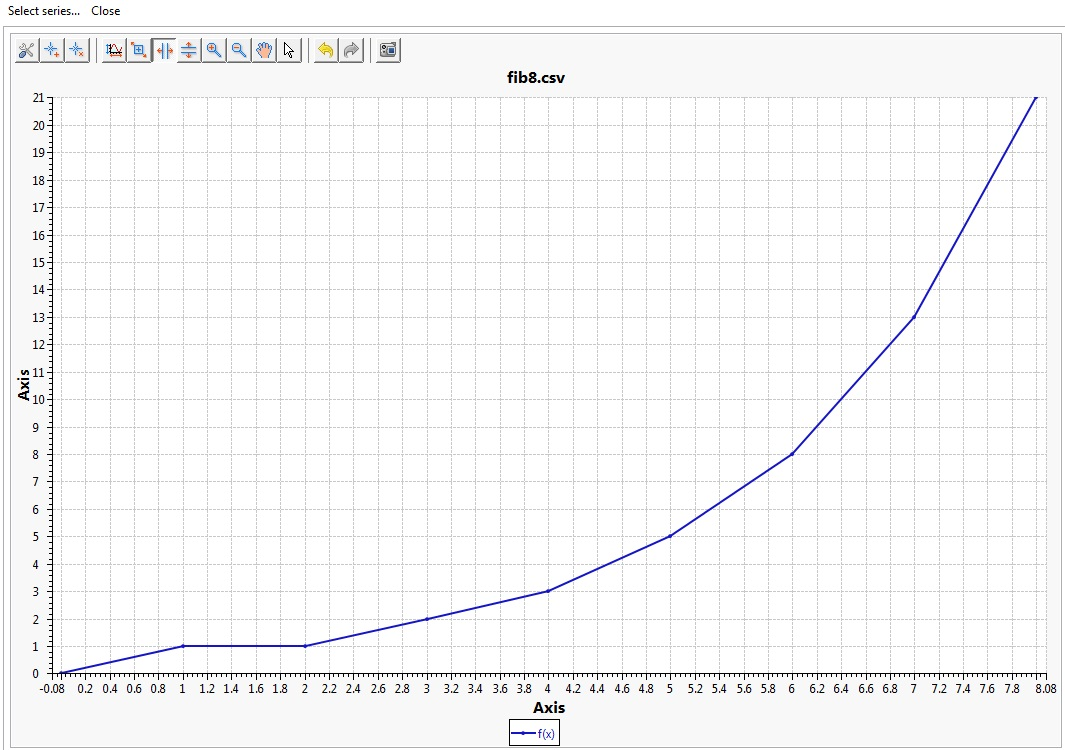
\includegraphics[width=12cm]{images/CSVPlotViewer}
\end{center}

\subsubsection{Controlling the Graphics}

The row of buttons at the top of the viewer provide basic graph editing
capabilities.

The first button allows the user to edit a variety of basic graph attributes,
such as font, axis titles and scales, line colors, etc.

The next two buttons allow for the addition and removal of annotations for
specific data points. 

The central grouping of buttons allow the user to zoom and pan the camera in a
variety of ways. 

The two yellow arrow buttons will undo/redo changes made to the graph.

The final button will export a screenshot of the graph.

\subsubsection{Setting the Independent Series}

By default, the first column in the file will serve as the independent series
setting the graph's x axis. By right clicking the Plot Viewer and selecting Set
Independent Series\ldots you can replace it with any other series in the file.

\subsubsection{Setting the Dependent Series}

When first opened, only the series defined by the second column in the file will
be displayed. There are several ways to change this. 

The Select Series\ldots button in the upper lefthand corer will display a list
of all the series in the file. Selecting one and pressing OK will graph that
series and removing all others.

Right clicking and choosing Select series\ldots from the context menu will open
a dialog in which any of the series will be selected. All selected series will
be graphed at once, with deselected series removed.

 

Finally, the Remove all series option in the context menu will completely clear
the graph.

\section{MOOSE Embedded Visualization}

MOOSE Workflow Items allow for easy visualization of their associated files,
making use of the VisIt and CSV Plot Editors described previously.

\subsection{Creating a MOOSE Workflow}

First open the MOOSE Perspective, either through Window $\rightarrow$
Perspective $\rightarrow$ Open Perspective $\rightarrow$ Other\ldots and
selecting MOOSE, or by clicking the Open Perspective button in the top right
corner and selecting MOOSE.

\begin{center}
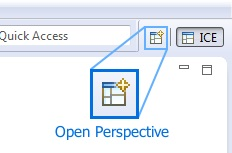
\includegraphics{images/ICE_OpenPerspective}
\end{center}

Next, you must open a MOOSE Workflow. The two buttons outlined in red below will
create Items. The upper one will import a .i file, while the bottom button will
create a new workflow. In either case, select MOOSE Workflow from the menu and
hit OK.

\begin{center}
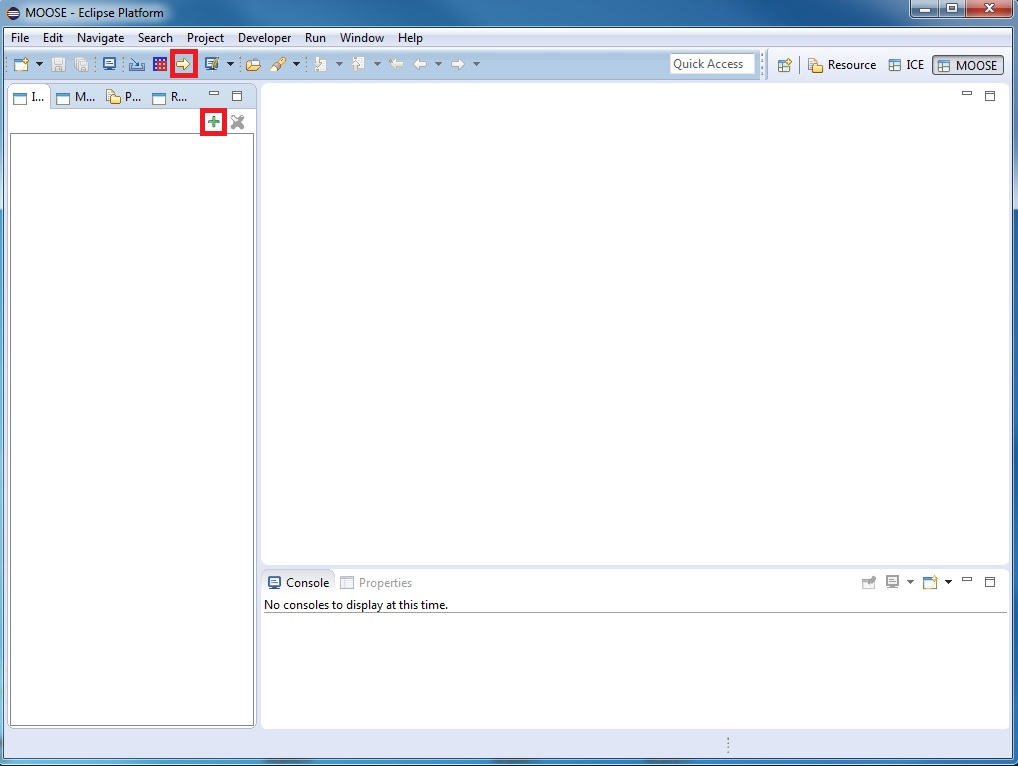
\includegraphics[width=12cm]{images/MOOSEPerspectiveNewWorkflow}
\end{center}

You must now choose the MOOSE application which will run the file. The
Browse\ldots button under MOOSE-Based Application in the upper left hand corner
will open a menu asking if the application is on the local machine or on a
remote one. For local applications, you will simply need to select it from a
dialog. 

\begin{center}
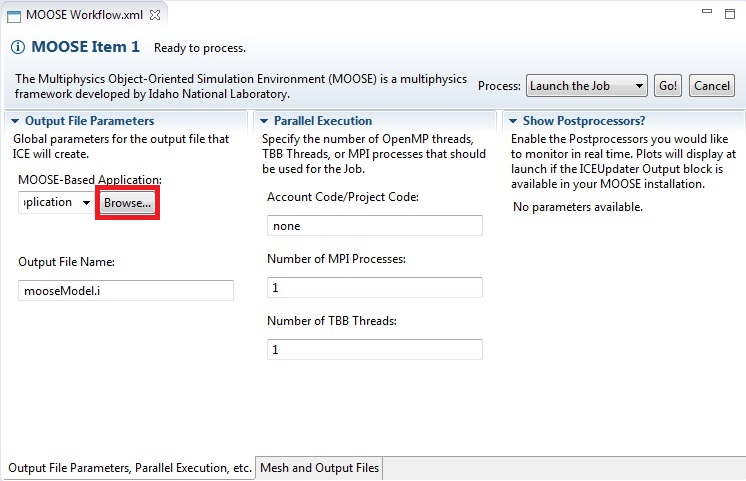
\includegraphics[width=12cm]{images/MOOSEItem}
\end{center}

If the application is remote, a new dialog will open. At the top, press the New
button to set up your connection. 

\begin{center}
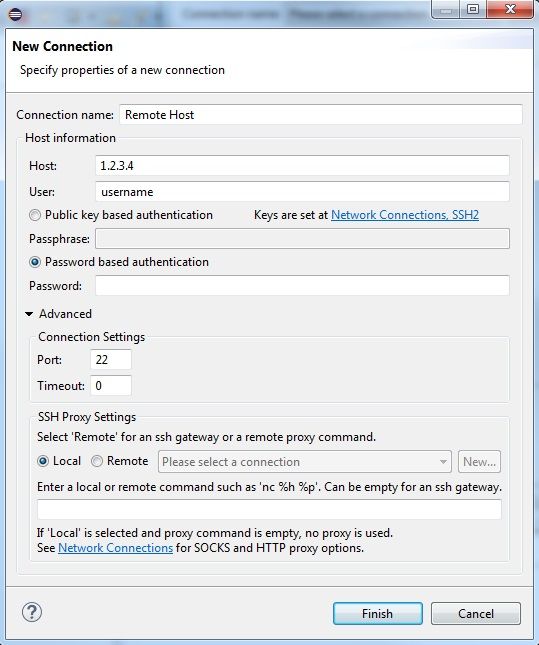
\includegraphics[width=12cm]{images/NewConnectionDialog}
\end{center}

You must set the Host to the computer containing the MOOSE application, and User
and Password to the username and password for your account on that machine. You
may also optionally set the Port number, timemout, and proxy settings. Once
done, click Finish. You will automatically be shown the file system for your new
connection. Select the MOOSE application from it and click OK.

Save the form. If you imported a file, there will still be unsaved changes after
a single save. You can save again and skip the next section. 

\subsubsection{Configuring the MOOSE Input Data}

\begin{center}
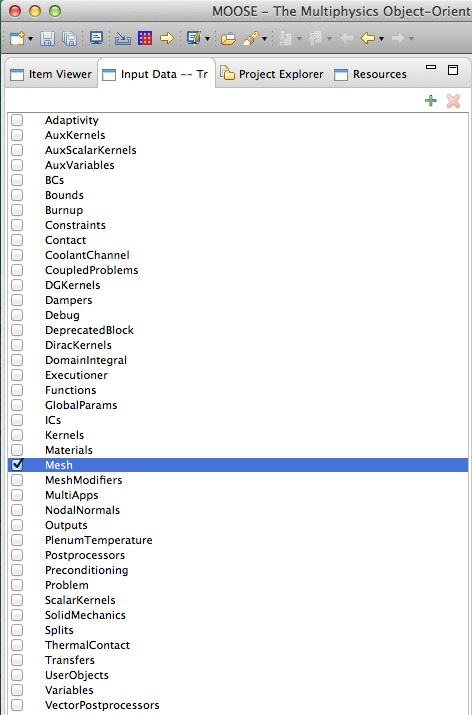
\includegraphics[width=6cm]{images/MOOSETree} 
\end{center}

If you did not import a pre-written MOOSE file, some setup will be
required before the job can create visualizations. Switch to the Input Data --
Tree View tab on the left of the screen. Here you will see a list of MOOSE data
categories. Click Mesh and switch to the Properties tab at the bottom.

\begin{center}
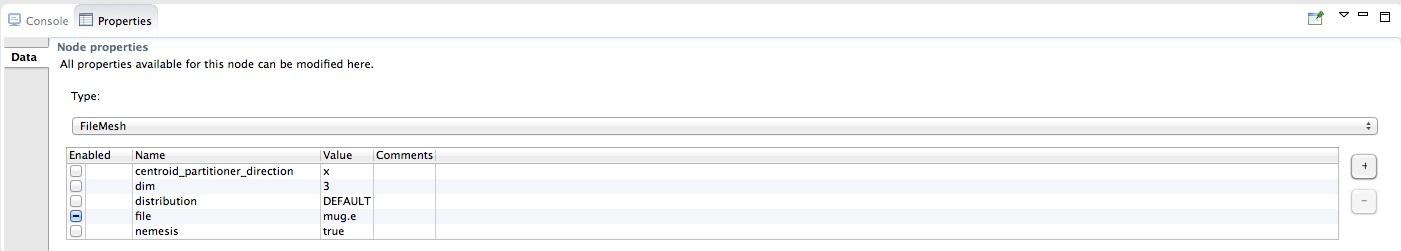
\includegraphics[width=12cm]{images/MeshProperty} 
\end{center}

The Properties tab will display the properties of the Mesh variable. At the top
will be drop down menu labeled Type. Select FileMesh from it and the table below
it will be populated. In the table, select the file line and place the file
containing the mesh you want to work with in it, as mug.e is in the example
above.

If there are any variables you want to graph from the job, you will have to
specify them as Variables and create PostProcessors which point to them,
similar to how you just set the Mesh. 

\subsection{Viewing the Embedded Visualizations} 

Once your MOOSE Workflow is set up, make sure the Process control is set to
``Launch the Job", and click the Go! button in the upper right hand corner. Wait
until the console shows that the output files are finished downloading, similar
to what is seen here:

\begin{center} 
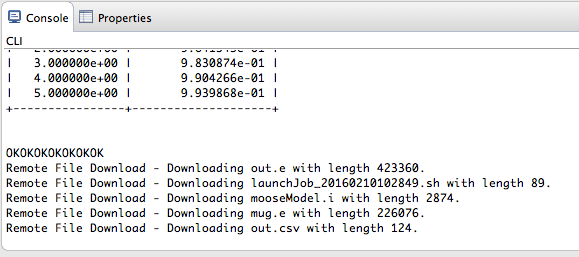
\includegraphics[width=12cm]{images/MOOSEJobConsoleOutput} 
\end{center}

You can now change to the Resources tab on the left. This will list all the
output files produced by the MOOSE job. Double clicking on one will open a Plot
Editor inside the MOOSE Item's Mesh and Output Files tab. The visualization can
be controlled normally, as described in previous sections.  

Multiple resources can be opened at once. At the top of the screen are controls
for the number of rows and columns making up the grid. These can be changed to
set the layout for the various plots, as demonstrated below.

\begin{center}
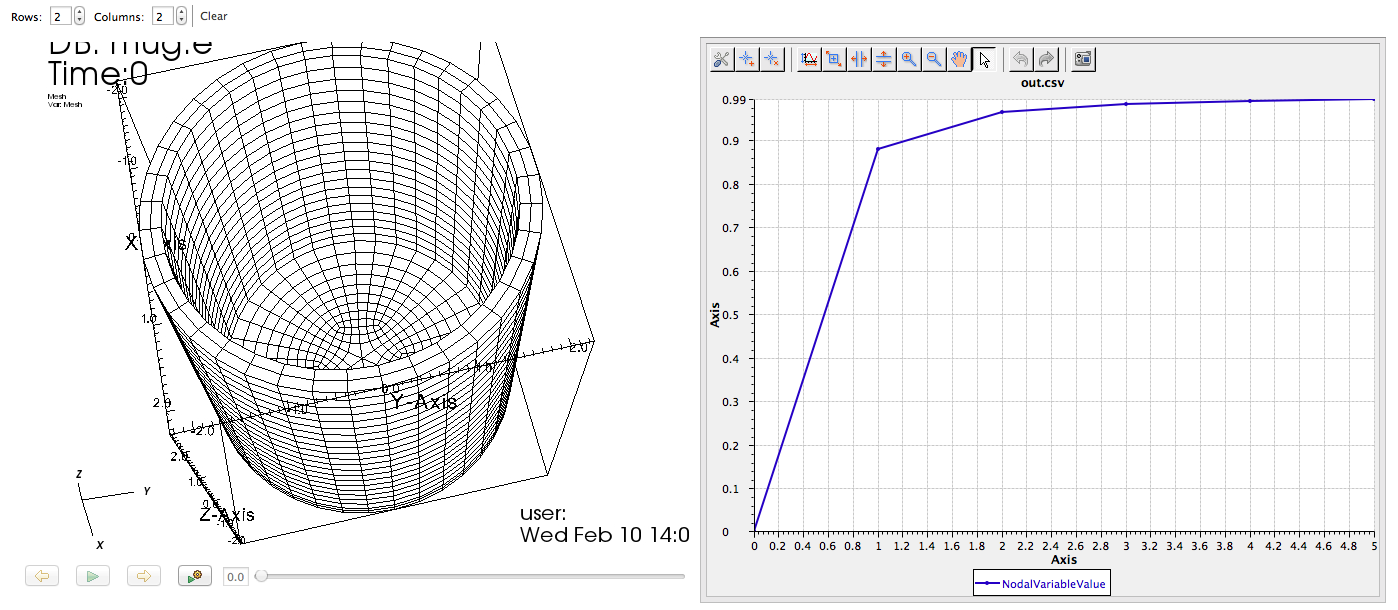
\includegraphics[width=12cm]{images/MOOSEEmbeddedHorizontal}
\end{center}

\begin{center}
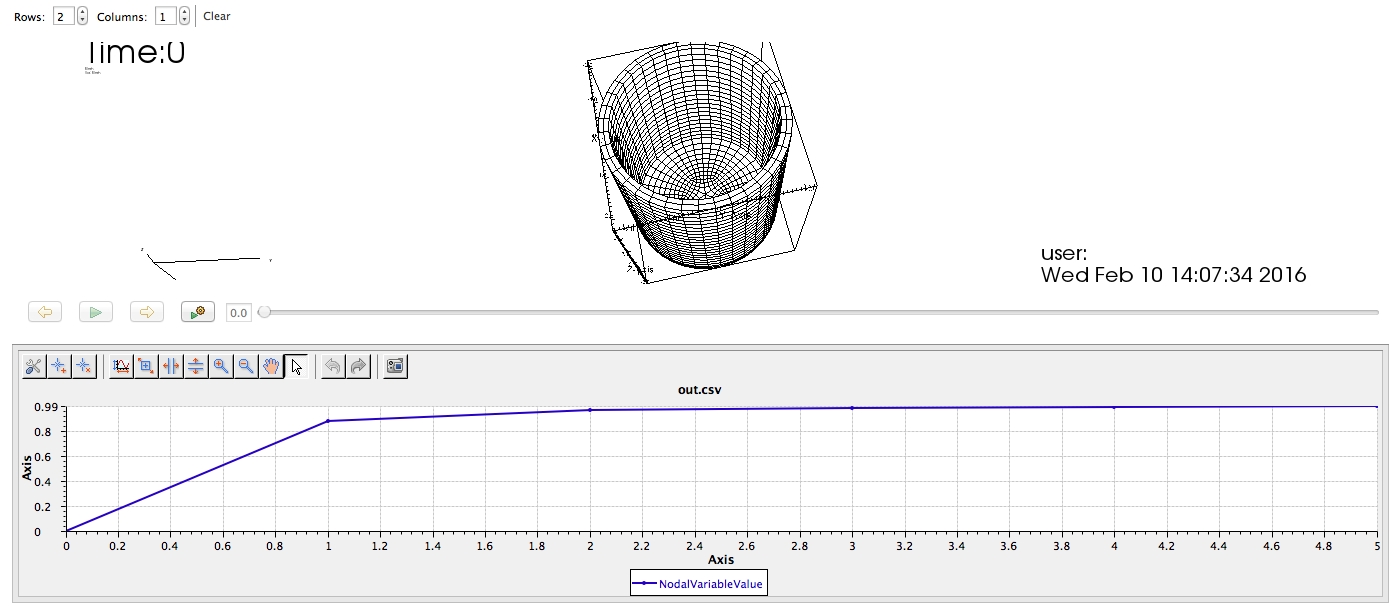
\includegraphics[width=12cm]{images/MOOSEEmbeddedVertical}
\end{center}

Be careful when reducing the number of rows or columns, as any plots which no
longer fit in the grid will be closed.

If you hover over a plot, a button will appear in the upper left hand
corner. Clicking it will close that plot.

\begin{center}
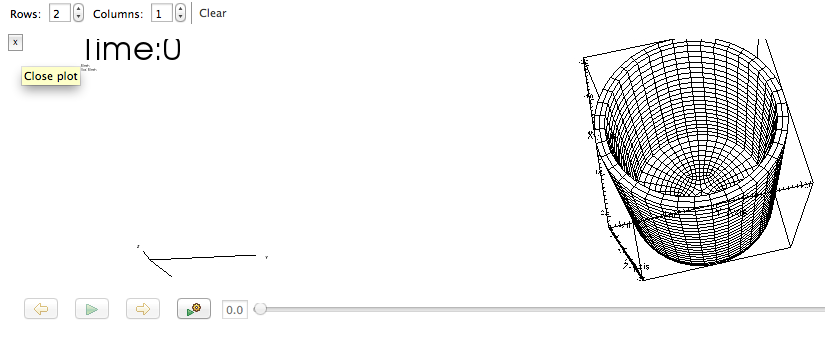
\includegraphics[width=12cm]{images/ClosePlotButton}
\end{center}

Alternatively, the Clear button next to the controls for the number of rows and
columns will close all the plots.

\end{document}

